%----------------------------------------------------------------------------------------
%       PACKAGES AND OTHER DOCUMENT CONFIGURATIONS 
%----------------------------------------------------------------------------------------
\documentclass[paper=letter, fontsize=12pt]{article}

\makeatletter
\newcommand*{\rom}[1]{\expandafter\@slowromancap\romannumeral #1@}
\makeatother
\usepackage{verbatim}
\usepackage[english]{babel} % English language/hyphenation
\usepackage{amsmath,amsfonts,amsthm} % Math packages
\usepackage[utf8]{inputenc}
\usepackage{float}
\usepackage{lipsum} % Package to generate dummy text throughout this template
\usepackage{blindtext}
\usepackage{graphicx} 
\usepackage{caption}
\usepackage{subcaption}
\usepackage[sc]{mathpazo} % Use the Palatino font
\usepackage[T1]{fontenc} % Use 8-bit encoding that has 256 glyphs
\linespread{1.05} % Line spacing - Palatino needs more space between lines
\usepackage{microtype} % Slightly tweak font spacing for aesthetics
\usepackage[hmarginratio=1:1,top=32mm,columnsep=20pt]{geometry} % Document margins
\usepackage{multicol} % Used for the two-column layout of the document
%\usepackage[hang, small,labelfont=bf,up,textfont=it,up]{caption} % Custom captions under/above floats in tables or figures
\usepackage{booktabs} % Horizontal rules in tables
\usepackage{float} % Required for tables and figures in the multi-column environment - they need to be placed in specific locations with the [H] (e.g. \begin{table}[H])
\usepackage{hyperref} % For hyperlinks in the PDF
\hypersetup{colorlinks=true, 
linkcolor=blue, 
filecolor=magenta, 
urlcolor=blue,}
\urlstyle{same}

\usepackage{lettrine} % The lettrine is the first enlarged letter at the beginning of the text
\usepackage{paralist} % Used for the compactitem environment which makes bullet points with less space between them
\usepackage{abstract} % Allows abstract customization
\renewcommand{\abstractnamefont}{\normalfont\bfseries} % Set the "Abstract" text to bold
\renewcommand{\abstracttextfont}{\normalfont\small\itshape} % Set the abstract itself to small italic text
\usepackage{titlesec} % Allows customization of titles

\renewcommand\thesection{\Roman{section}} % Roman numerals for the sections
\renewcommand\thesubsection{\Roman{subsection}} % Roman numerals for subsections

\titleformat{\section}[block]{\large\scshape\centering}{\thesection.}{1em}{} % Change the look of the section titles
\titleformat{\subsection}[block]{\large}{\thesubsection.}{1em}{} % Change the look of the section titles
\newcommand{\horrule}[1]{\rule{\linewidth}{#1}} % Create horizontal rule command with 1 argument of height
\usepackage{fancyhdr} % Headers and footers
\pagestyle{fancy} % All pages have headers and footers
\fancyhead{} % Blank out the default header
\fancyfoot{} % Blank out the default footer

\fancyhead[C]{University Of California Berkeley $\bullet$ \date{\today} } % Custom header text

 \fancyfoot[RO,LE]{\thepage} % Custom footer text




 
%----------------------------------------------------------------------------------------
%       TITLE SECTION
%----------------------------------------------------------------------------------------
\title{\vspace{-15mm}\fontsize{24pt}{10pt}\selectfont\textbf{Final Project: Color Sensor}} % Article title
\author{
\large
{\textsc{\textbf{Jeffrey Vargas} }}\\[2mm]
{\textsc{Yash Sanjay SHAH }}\\[2mm]}
\date{\today}




%----------------------------------------------------------------------------------------
\begin{document}
\maketitle % Insert title
\thispagestyle{fancy} % All pages have headers and footers
%_----------------------------------- ------------------------------

%-------------------------------------------------------------------------------------------------------------------------------------------------------------------------------
%      									 Abstract
%-------------------------------------------------------------------------------------------------------------------------------------------------------------------------------


\section*{Abstract}

Analyzing the spectrum of objects is a common practice in many fields of science; however, sophisticated spectrometers can be expensive. As a result, we decided to take an elementary yet comprehensive, approach to spectroscopy. For our project we designed and constructed an inexpensive color sensor, whose function is an analogous to a spectrometer. We used a film canister with three colored LED's and a photo-diode mounted inside to measure the color of objects in the lab. By convention we chose the base colors for LED's to be Red, Blue and Green (RGB). Our results show that we can map measured voltages to color space, where color space is represented by the  standard 3X3 RGB matrix. 
\[
Y_{rgb} = 
\begin{bmatrix}
R & G & B\\ 
255 & 0 & 0\\ 
0 & 255 & 0\\ 
0 & 0 & 255\\ 
\end{bmatrix}
\]

Each column represent pure red, green and blue respectively.  We conclude that the basis matrix required to construct the transformation matrix is sensitive to noise; as a result, we amplified our signal which increased our signal to noise ratio. We also added capacitors in order to decouple any intrinsic noise. This allowed for a more accurate  color mapping. \\
  


%-----------------------------------------------------------------------------------------------------------------------------------------------------------------------------------------------------
%      									 Introduction
%-----------------------------------------------------------------------------------------------------------------------------------------------------------------------------------------------------

\section*{Introduction}
Analyzing the spectrum of objects is a common practice in many fields of science; however, sophisticated spectrometers can be expensive.As a result, we decided to take an elementary yet comprehensive, approach to spectroscopy. In our experiment we set out to measure the color of different objects by measuring the reflected and absorb photons, hence we built a color sensor. 

	Generally white light contains all colors visible to the eye; that is white light contains photons with a range of wavelength which the eye can interpret as different colors. However, while these wavelengths are coupled together we see it as white light. By using a prism we can break the white light into its components and distinguish the \textbf{\textit{visible light}} spectrum (Figure\ref*{prism}). 

	\begin{figure}[H]
	\centering
	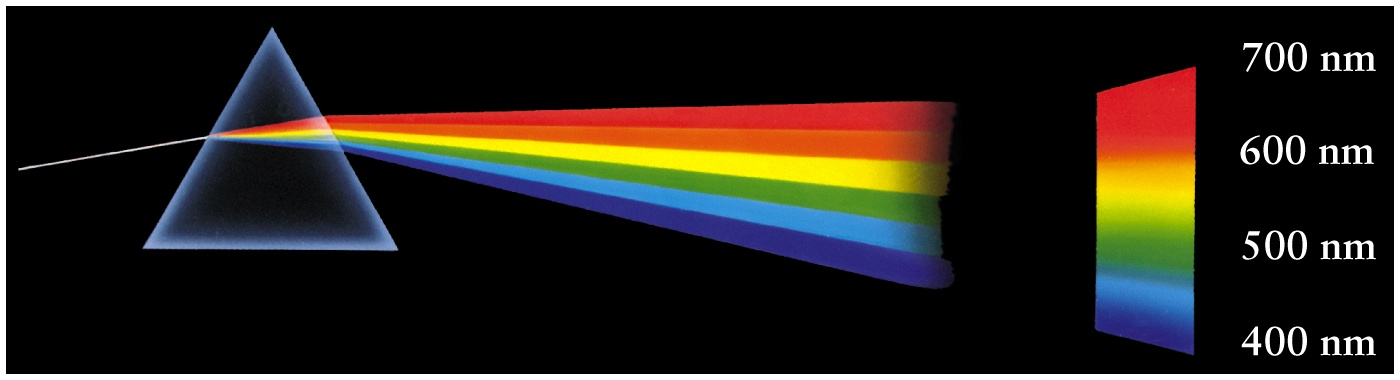
\includegraphics[scale=.4]{prism.jpg}
	\caption{visible light }
	\label{prism}
	\end{figure}

	Objects have different colors because their atoms can absorb or reflect light. For example, an object such as an apple, shines red because the atoms in the surface of the apple can absorb photons with wavelengths that do not correspond to the color red. Photons which have longer wavelength, i.e the color red, cannot be absorb by the surface of the apple and are therefore reflected. In other words, only photons with specific frequencies can be absorb. As a result, the atoms in objects can either absorb or reflect photons with different frequencies. The relation between frequencies and wavelength is given by, $c=\lambda \nu$, where $\lambda$ and $\nu$ are wavelength and frequency respectively. Absorption of photons occurs through resonance. When the frequency of the photon matches the resonance frequency of an object, then photon is absorb and the the object vibrates at that frequency. The energy of the photon stays in the object as thermal or vibrational energy and therefore the eye can no longer see that photon. If the light wave is instead reflected then the photons frequency did not math the resonant frequency of the object, therefore, the eye can capture the reflected photon and interpret it as a specific color (Figure \ref*{absorption and reflection}).

	\begin{figure}[H]
	\centering
	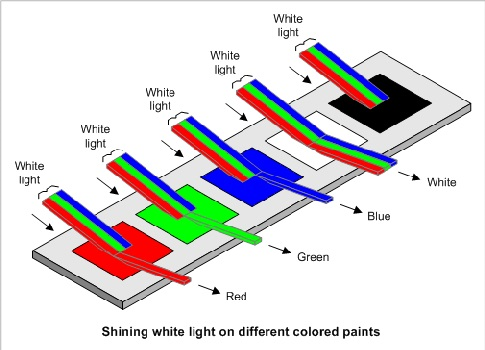
\includegraphics[scale=.6]{absorb_reflect2.png}
	\caption{absorption and reflection}
	\label{absorption and reflection}
	\end{figure}

	The color sensor we built essentially operates under this property of light, \textit{absorption} and \textit{ reflection}.\\


%----------------------------------------------------------------------------------------
%      							Instrument 	
%----------------------------------------------------------------------------------------


\section*{Instrument}

\subsection*{Theory}

In order to make use of the absorption and reflection of light our circuit had to be able to take in information from light at different frequencies. We decided to use a photo-diode to measure any light information we collected. we also used an op-amp to amplify our measured light signals. 

Measuring wavelengths or frequencies using a photodiode is not practical. This is because our analog to digital converter (DAC) is not capable of reading frequencies at the visible light scale, 430–770 THz!. Instead, we used the property of diodes to extract light information.Photodiodes, as the name implies, is a diode with P-N junction therefore in order to produce current, electron hole pairs must be filled. The photo-diode forms these pairs by absorbing photon which have an energy greater than the specified band gap energy (for \textit{Si} its 1.1ev ) and transmits that into current. As a result, the photodiode can absorb photons with a range of frequencies. The problem here is identifying the photons which produced the current.

We however, took a clever approach to the problem by specifying which colors should be absorb. We chose three LED's, naturally red, green and blue, and surrounded the photodiode with these LED's inside a film canister. This allowed us to see how much red, green, and blue is being reflected or absorb. It also allowed us to construct a 3X3 basis matrix of measured voltage amplitudes. The basis matrix was constructed by measuring the voltage amplitudes of pure red, green and blue and placing those values into the columns of the basis matrix. Finally, after digitizing the analog information we did some data processing using \textit{labview} and obtained the color information we wanted (see \textbf{Software} section).\\

\subsection*{circuit}

The circuit was composed of three 555 timers. The resistors and capacitors for the 555 timers where chosen such that the voltage output had frequencies of 1kHz, 2kHz and 4kHz. Each frequency was assigned to a specific LED. The red LED had 1kHz, the green had 2kHz, and the blue had 4kHz. This resulted in the LED's flashing at those specific frequencies. The purpose of this was to distinguish the LED's after reading in the information into Labview. The circuit diagram of the 555 timers is given in figure \ref*{timer}

	\begin{figure}[H]
	\centering
	\includegraphics[scale=.6]{555timer_1kHz.png}
	\caption{555timer}
	\label{timer}
	\end{figure}

\begin{tabular}{ |p{3cm}||p{3cm}|p{3cm}|p{3cm}|  }
 \hline
 \multicolumn{4}{|c|}{555 timers resistor and capacitor values} \\
 \hline
 			&  Red $\approx$ 1kHz	& Green $\approx$ 2kHz	& Blue $\approx$ 4khz\\
 \hline
 resistor 1  & 	6.8k$\Omega$	& 9.1k$\Omega$			& 		4.7k$\Omega$	\\
 \hline
 resistor 2  & 	68k$\Omega$		& 	33k$\Omega$			& 		15k$\Omega$		\\
 \hline
 capacitor   & 	10nF			& 	10nF				& 		10nF			\\

 \hline
 \hline
\end{tabular}\\
\\

Next we added an opamp to our circuit. The photodiode works by creating photons into current however lab computers and the the Digital to analog converter, DAC, works best when reading in voltage. Since the opamp is essentially a \textit{perfect} current to voltage converter we used an opamp with a 1M$\Omega$ resistor to convert and amplify the signals produced by the LED's. We also used a 1k$\omega$ resistor before the the photodiode which create a voltage divider and assisted in amplifying the signal. The circuit is shown in figure \ref*{amplify}. 



	\begin{figure}[H]
	\centering
	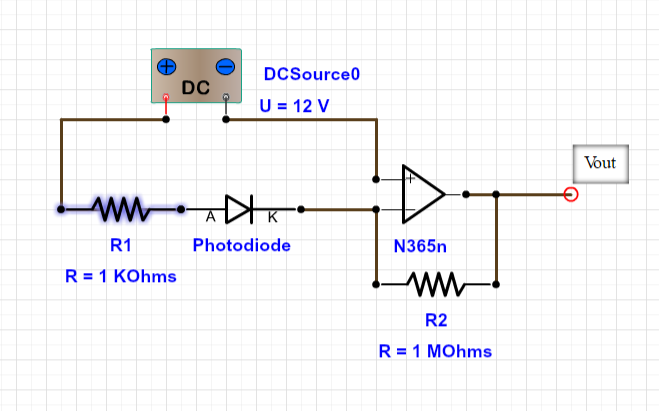
\includegraphics[scale=.6]{amplify.png}
	\caption{Opamp}
	\label{amplify}
	\end{figure}

	Finally we used .1$\mu$F capacitors to decouple the intrinsic noise in the circuit. Finally we grounded the 555 timers and the opamp separately to get rid of noise. 


\begin{figure}[H]
\centering
\begin{minipage}{.3\textwidth}
  \centering
  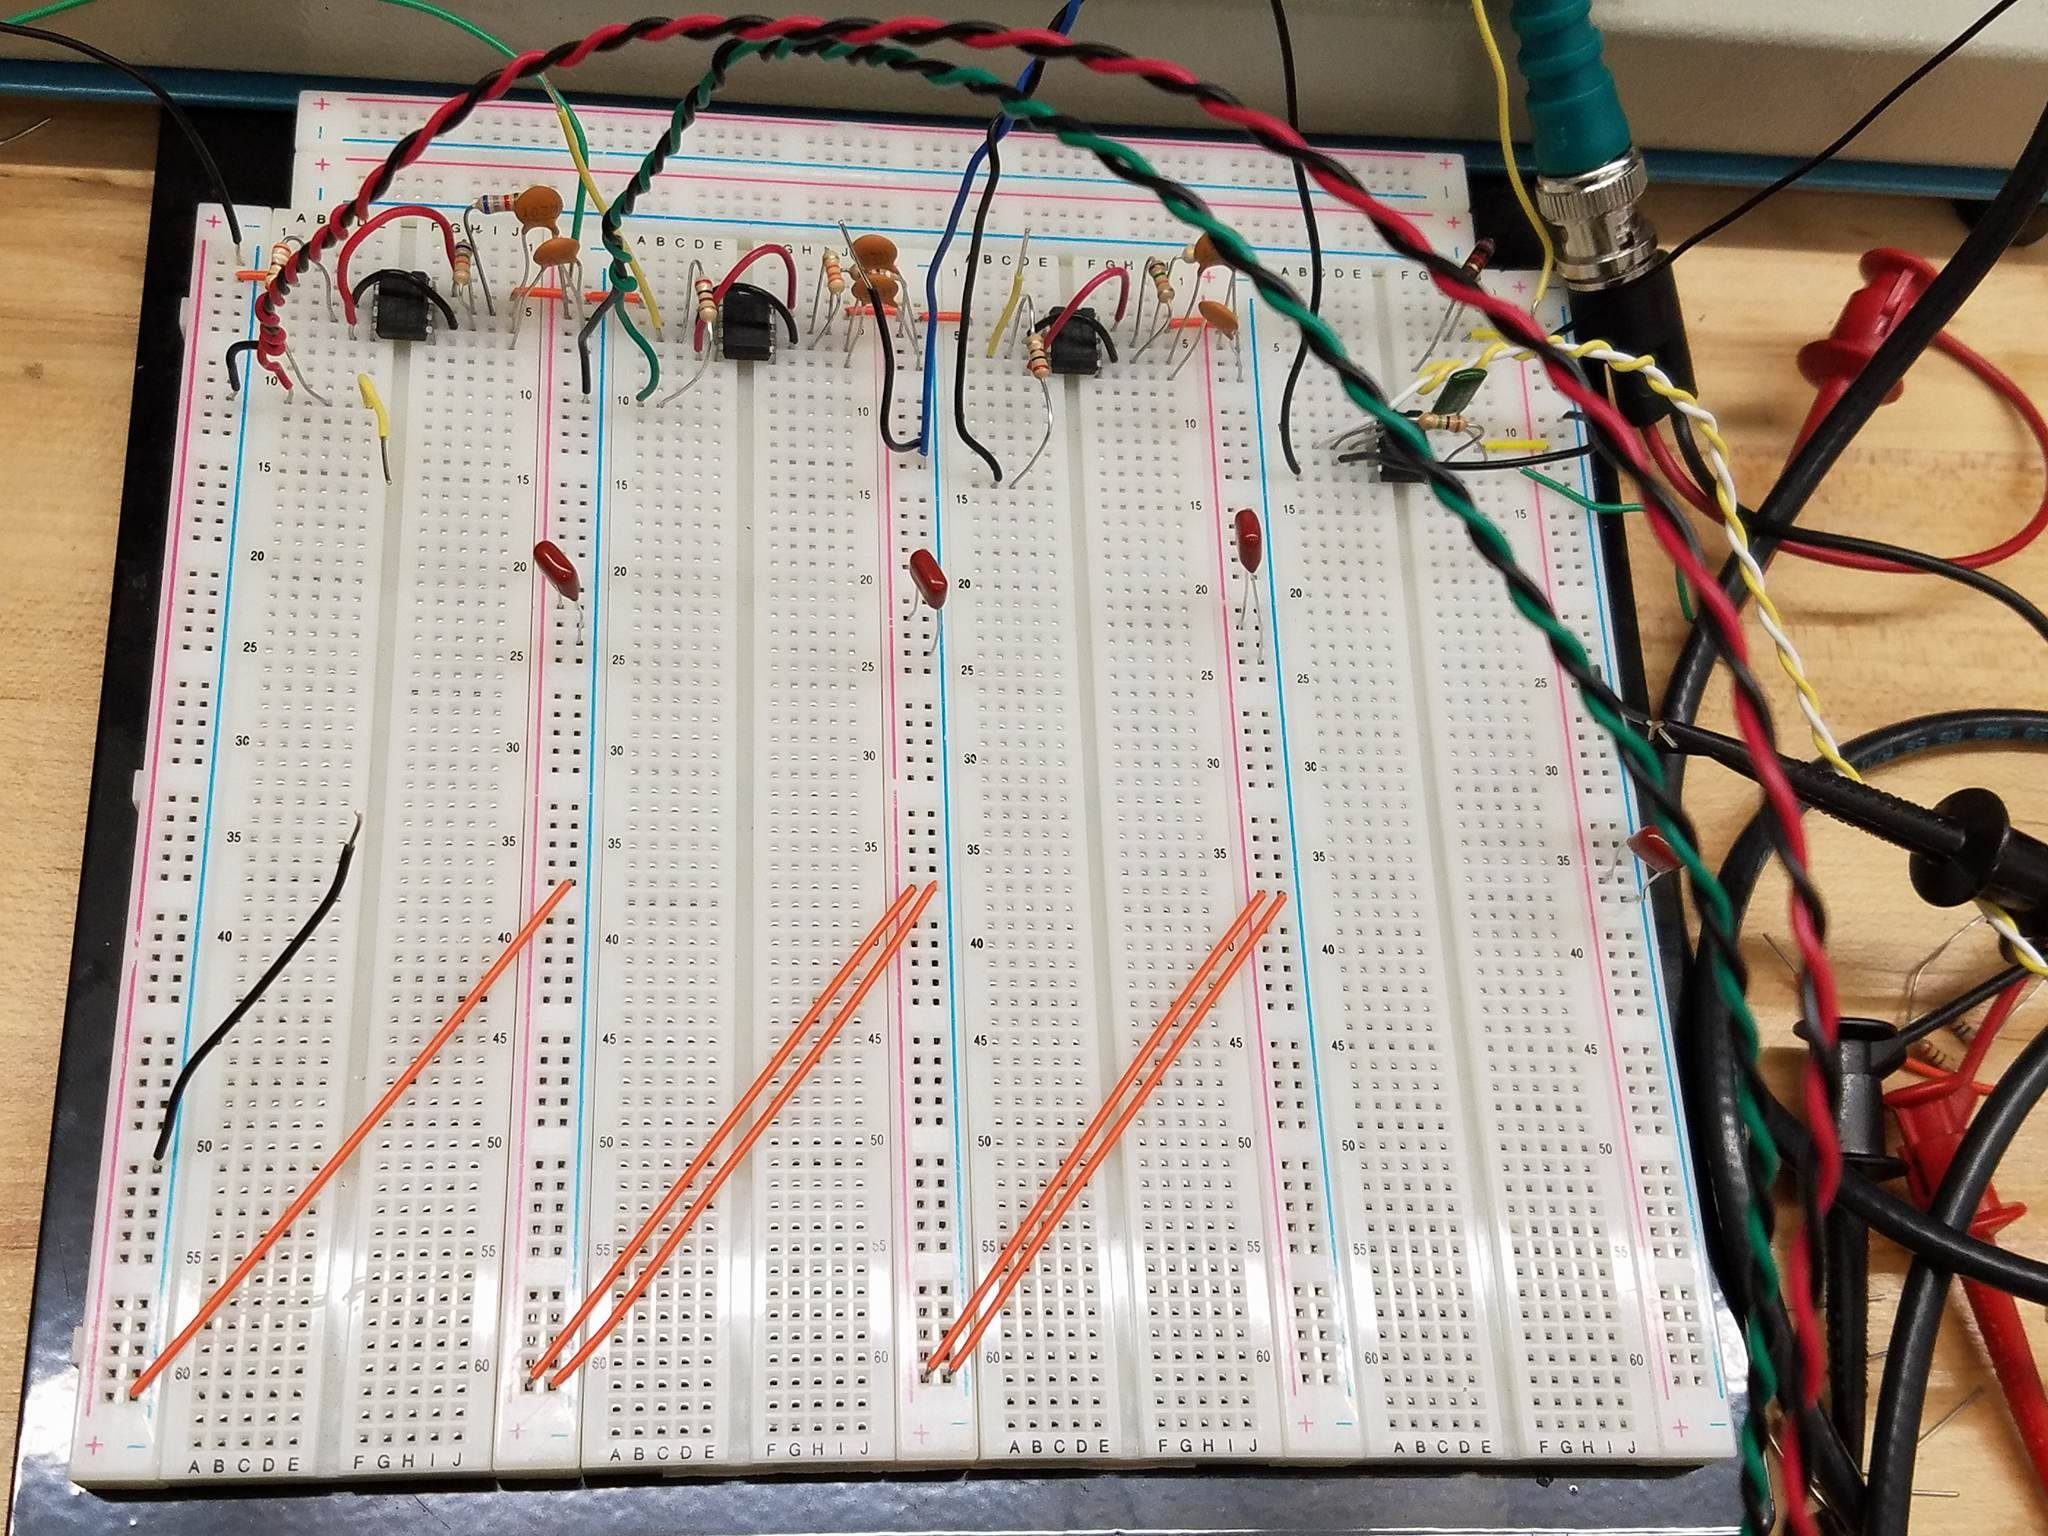
\includegraphics[width=.99\linewidth]{rawcircuit.jpg}
  \captionof{figure}{Circuit}
  \label{rawcircuit}
\end{minipage}%
\begin{minipage}{.3\textwidth}
  \centering
  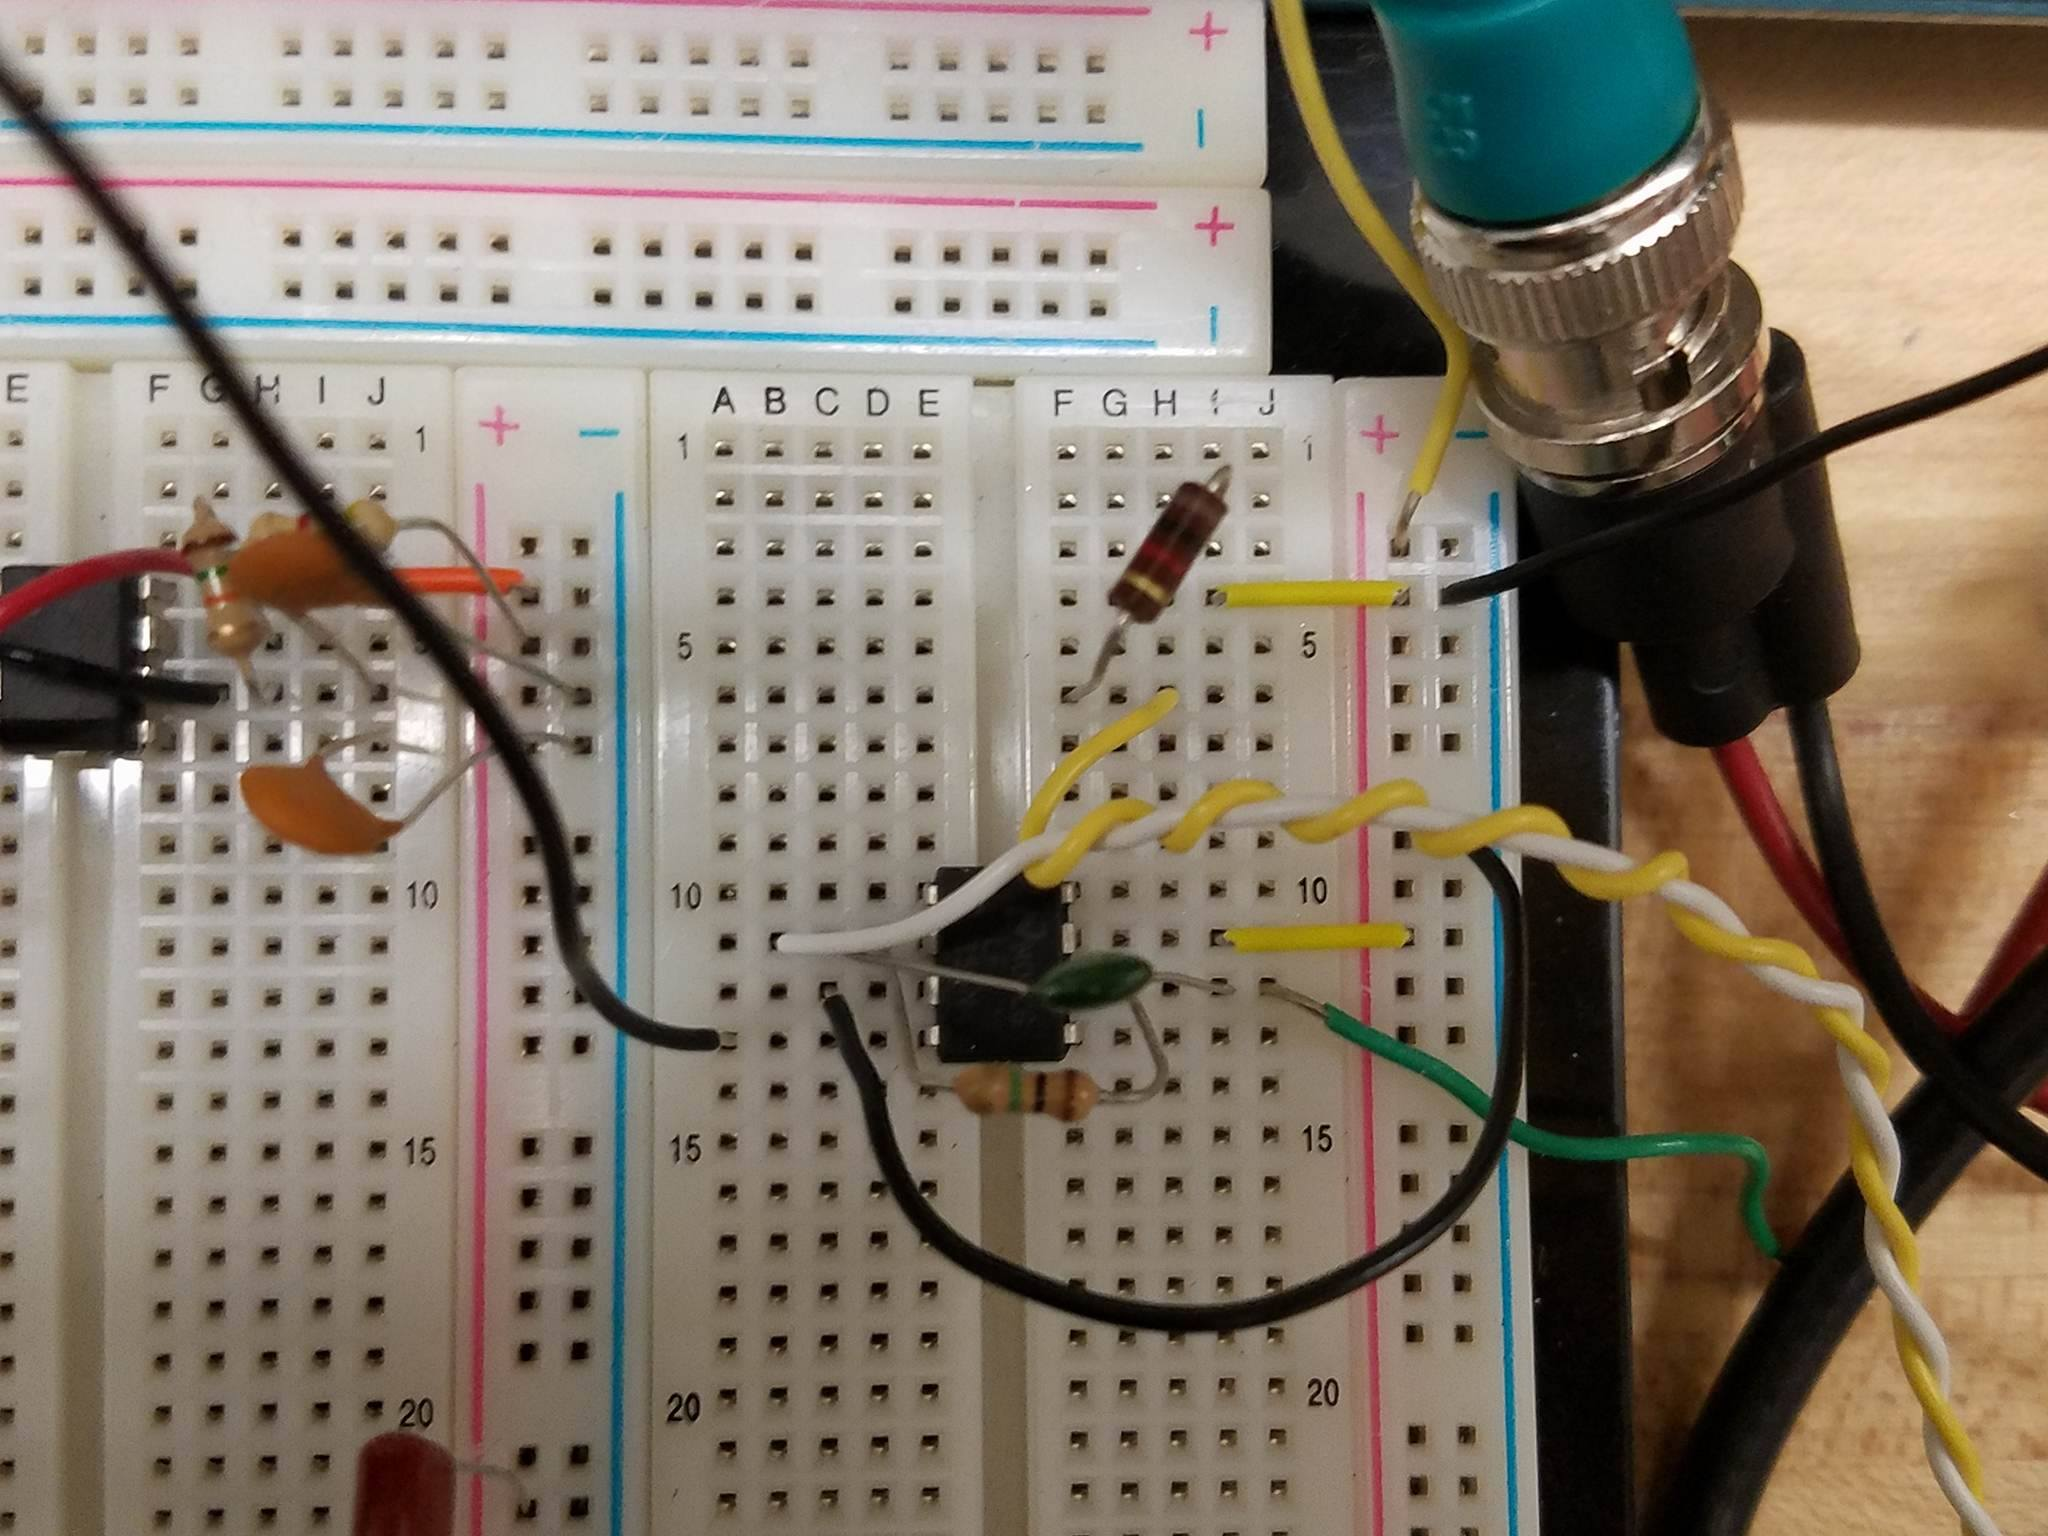
\includegraphics[width=.99\linewidth]{rawopamp.jpg}
  \captionof{figure}{Opamp}
  \label{rawopamp}
\end{minipage}%
\begin{minipage}{.3\textwidth}
  \centering
  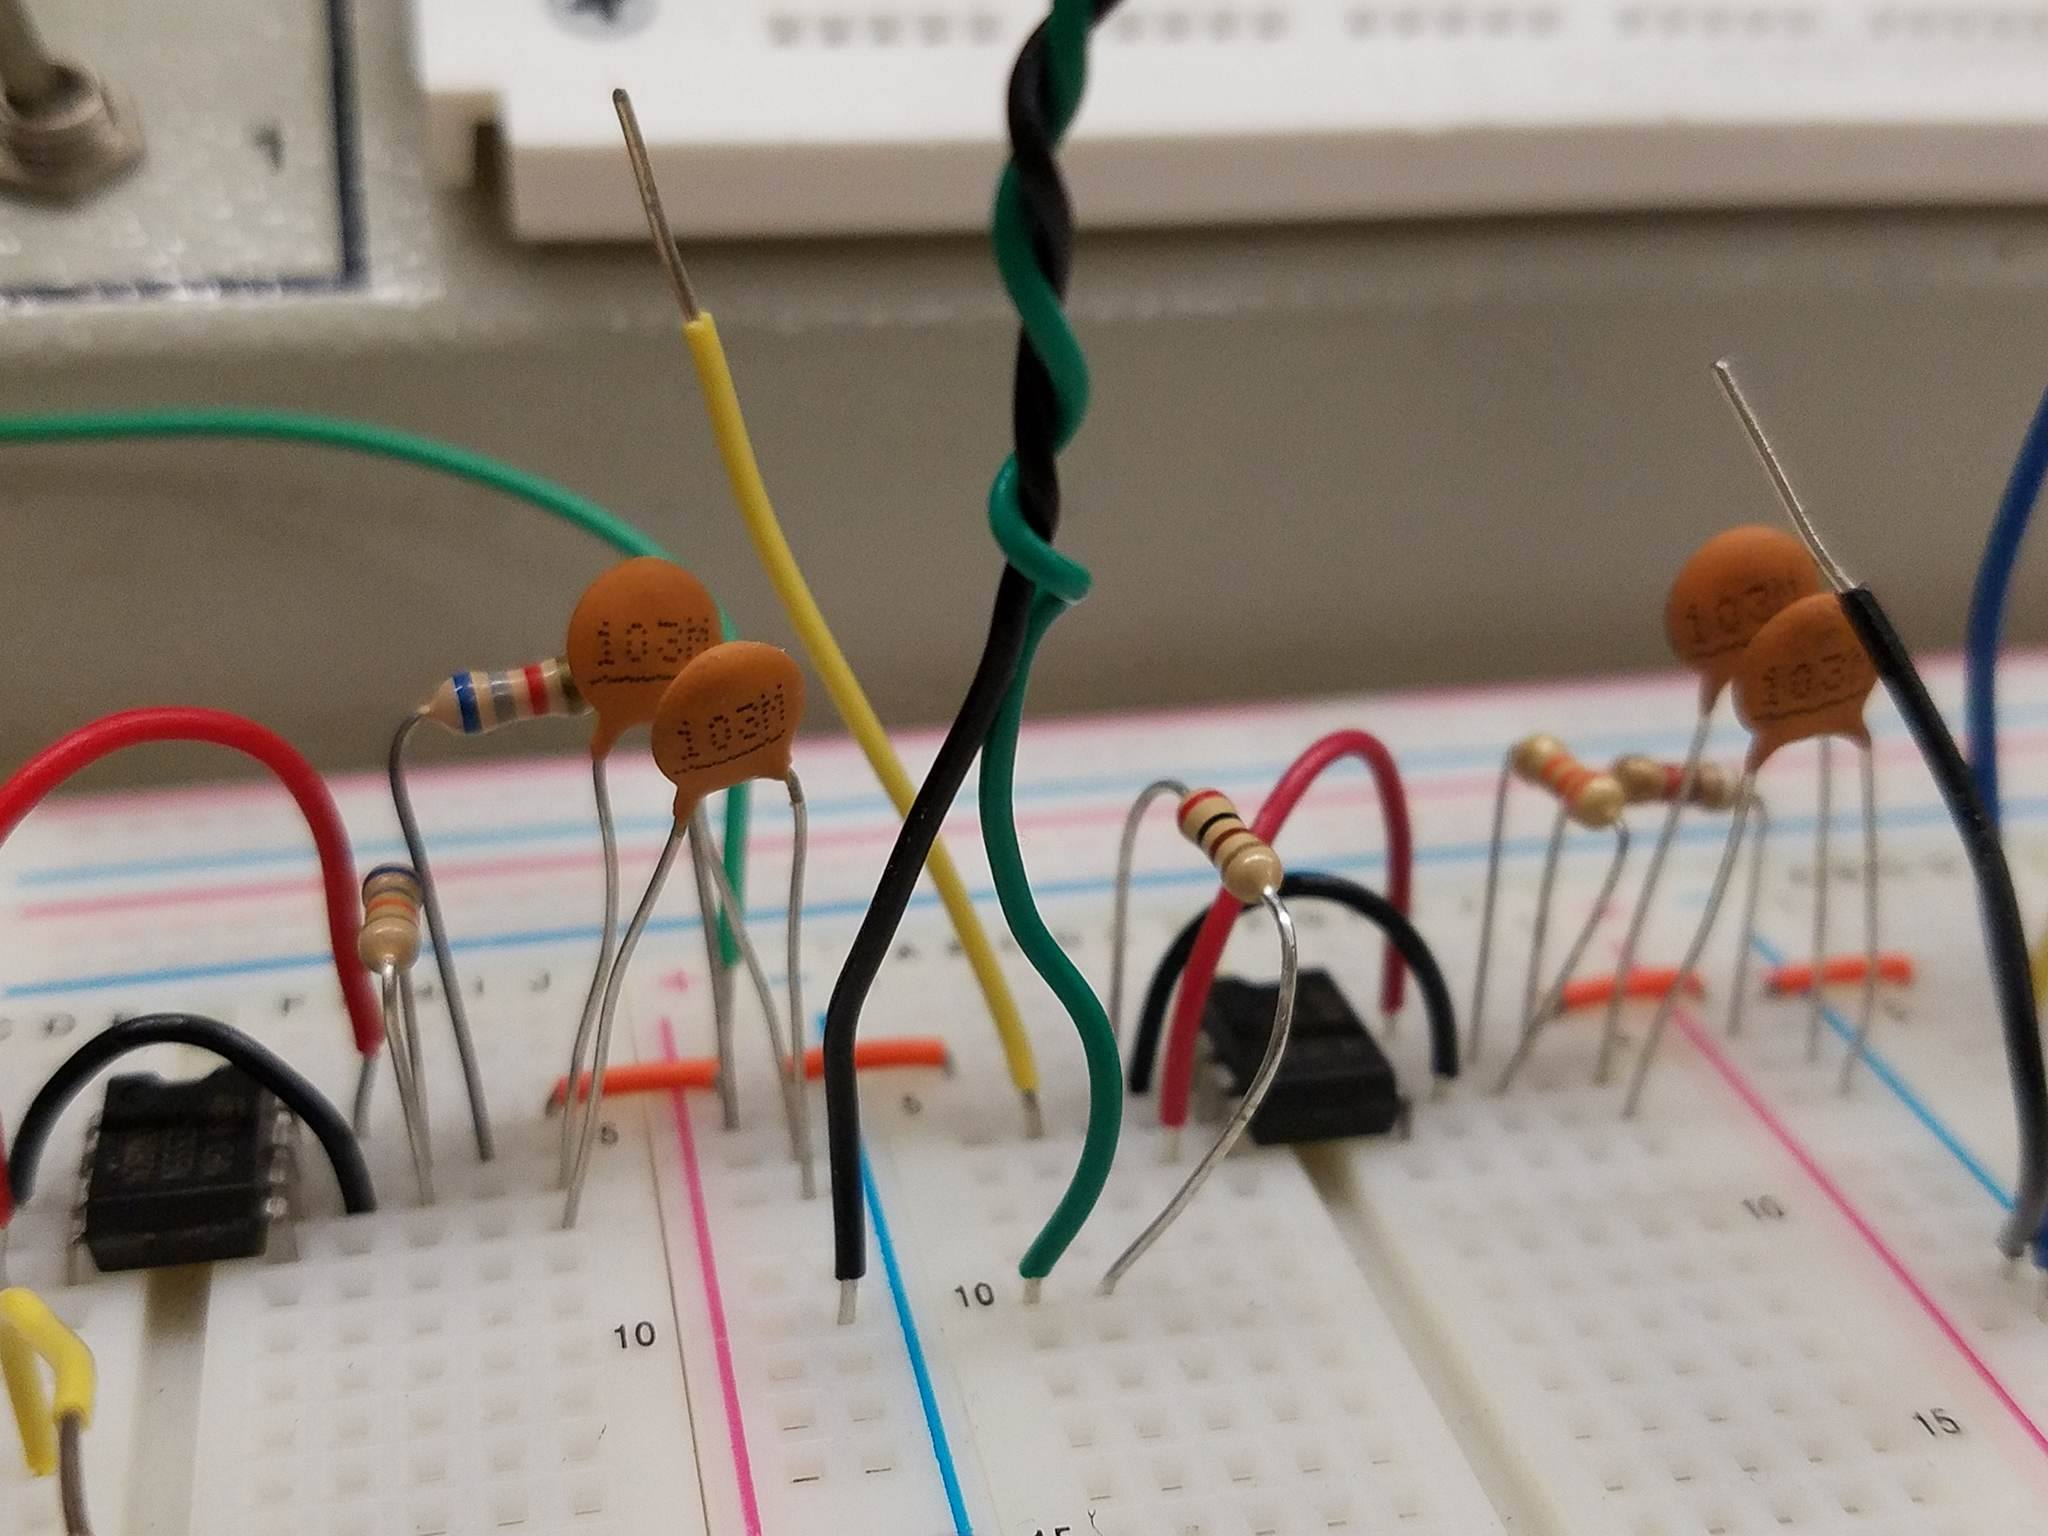
\includegraphics[width=.99\linewidth]{rawtimers.jpg}
  \captionof{figure}{1k and 2k timer}
  \label{rawtimers}
\end{minipage}
\end{figure}


%The Final image, Figure \ref*{filmcanister} is the film canister we used with the RGB LED's mounted inside and the photodiode at the center of the LED's.

\begin{figure}[H]
	\centering
	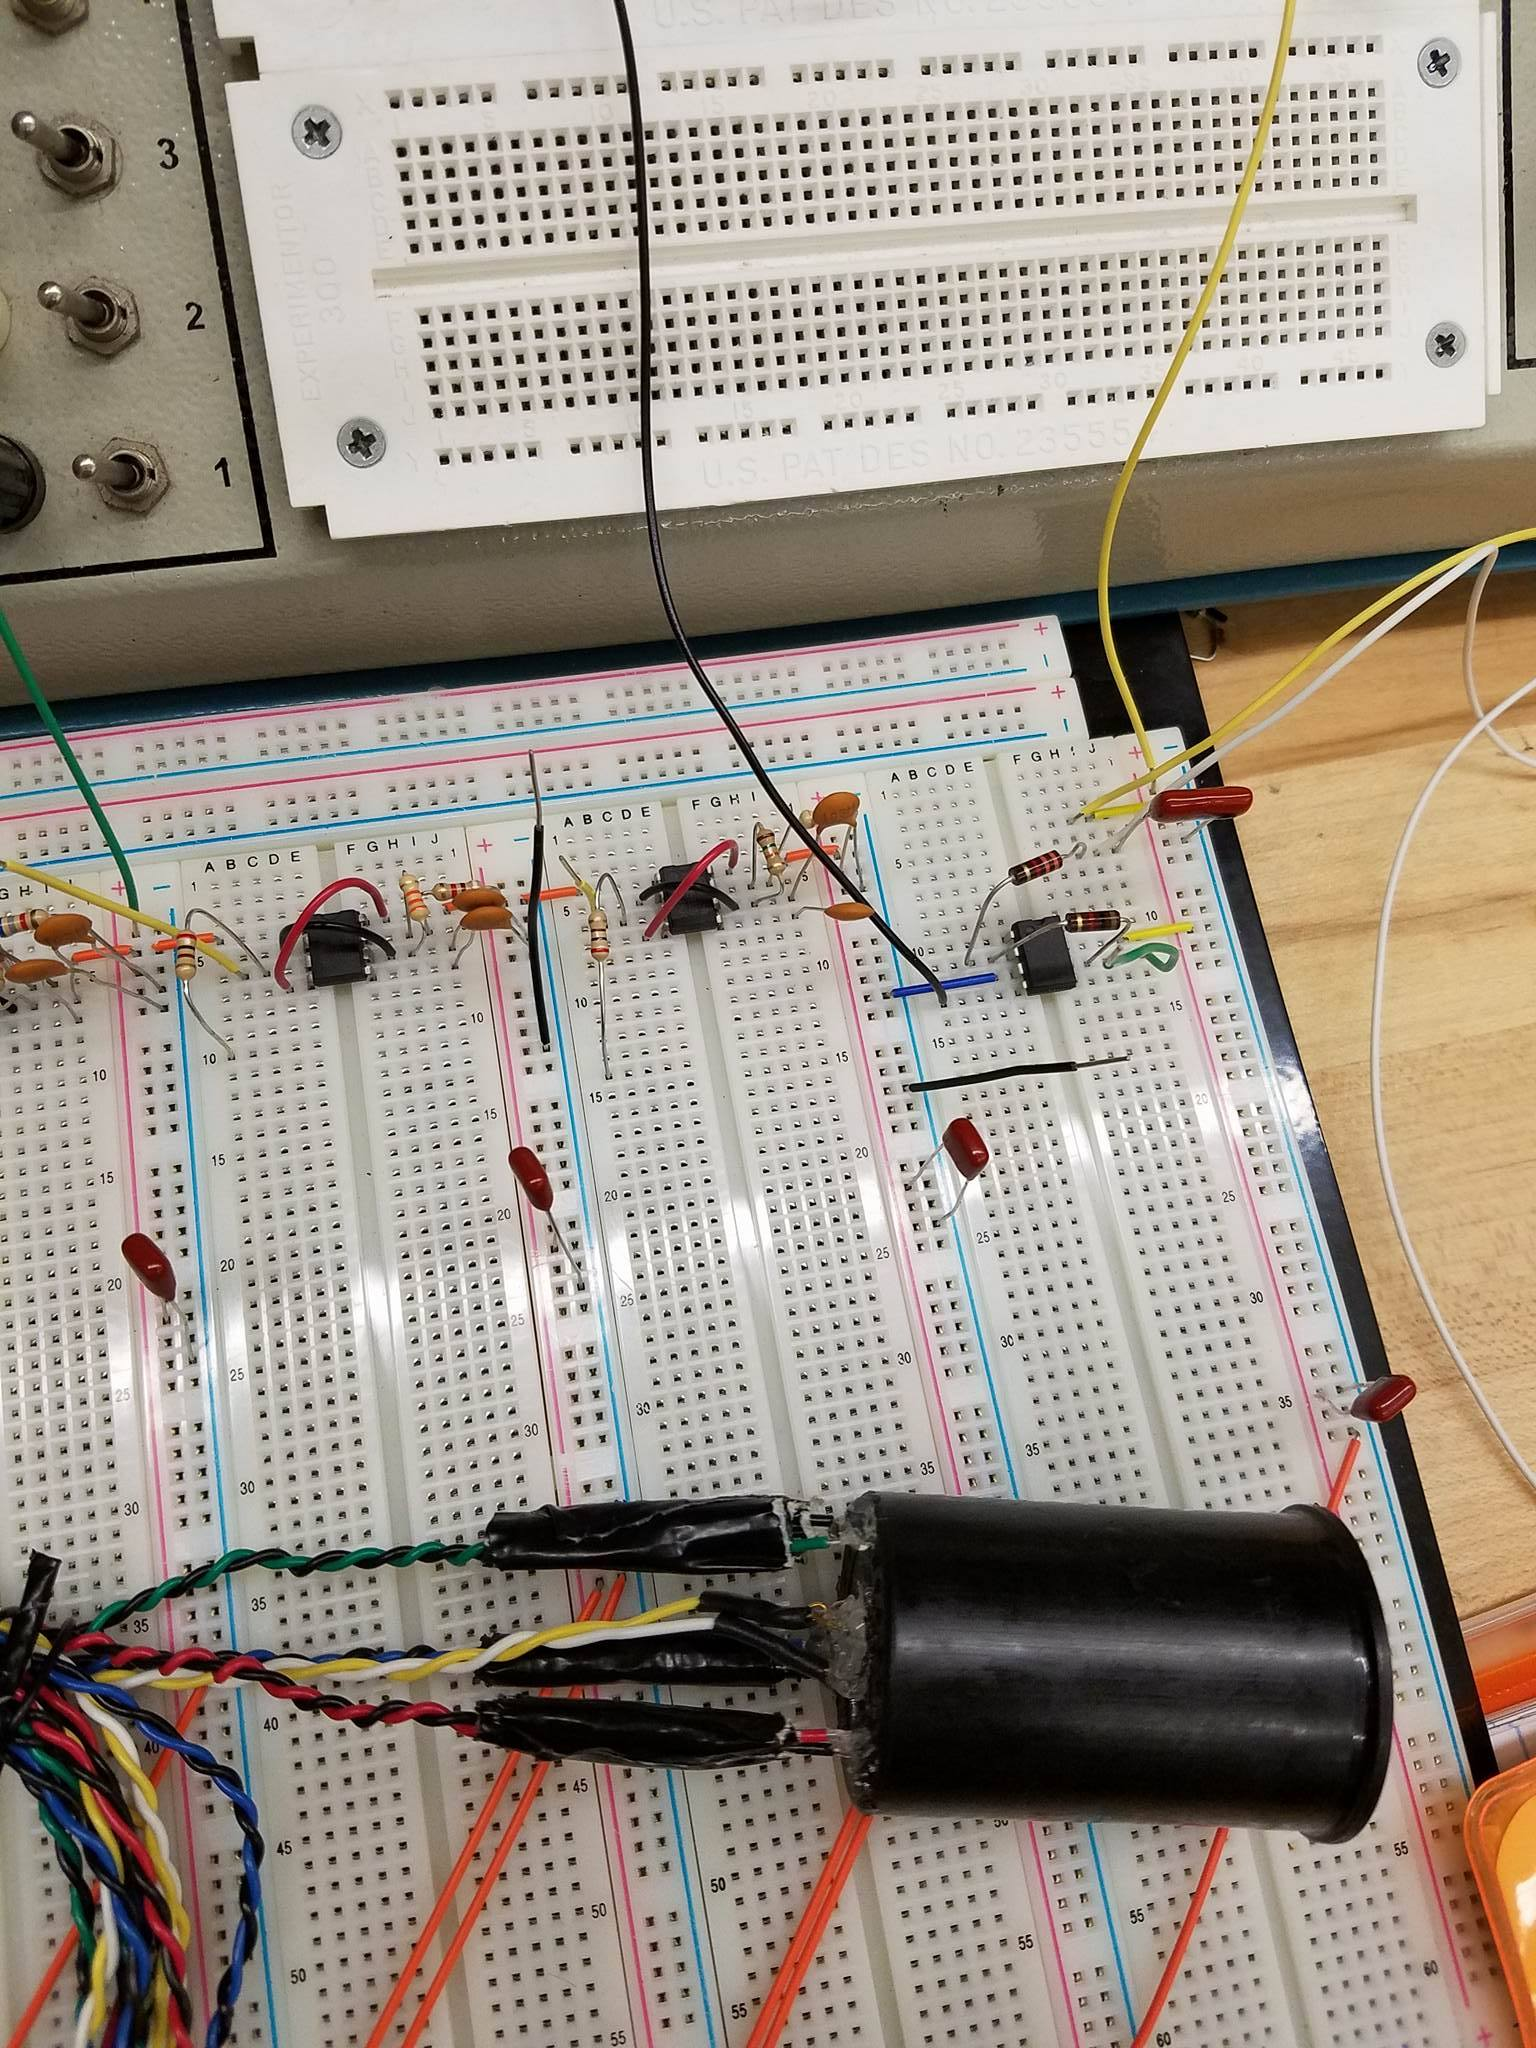
\includegraphics[scale = .09]{filmcanister.jpg}
	\caption{film canister with LED's and photodiode mounted inside.}
	\label{filmcanister}
\end{figure}

\section*{Software}

Our circuit produces analog signals in the form voltages which can be read using the DAQ in the LAB, however, in order to extract information we used Labview to process the data. The purpose of our Labview program is to read in the analog signals and and process the data. After processing the data we will be able to determine the amount of red green and blue object has, hence we will determine its color.

First we used the built in DAQ assistant function to read in the voltages into labview. The setting in the DAQ function were set to read 2k samples at a rate of 10kHz. Initially we could not Visually distinguish the voltages of the RGB LED's to that of noise because the voltage information is collected overtime as seen in the time stream graph in Figure \ref*{front}. As a result, if we wanted to see the voltage amplitudes that corresponded to the LED's we had to analyze the information in the frequency Domain. This required a Fourier transform of the signal. doing this we transformed the information and we could now display it using another waveform graph. The new graph displayed voltages vs frequency. A built in Labview function called spectral measurement allowed us to easily do the Fourier transform. Figure \ref*{front} shows how the LED's voltage amplitude occur at approximately 1kHz, 2kHz, and 4kHz.

\begin{figure}[H]
\centering
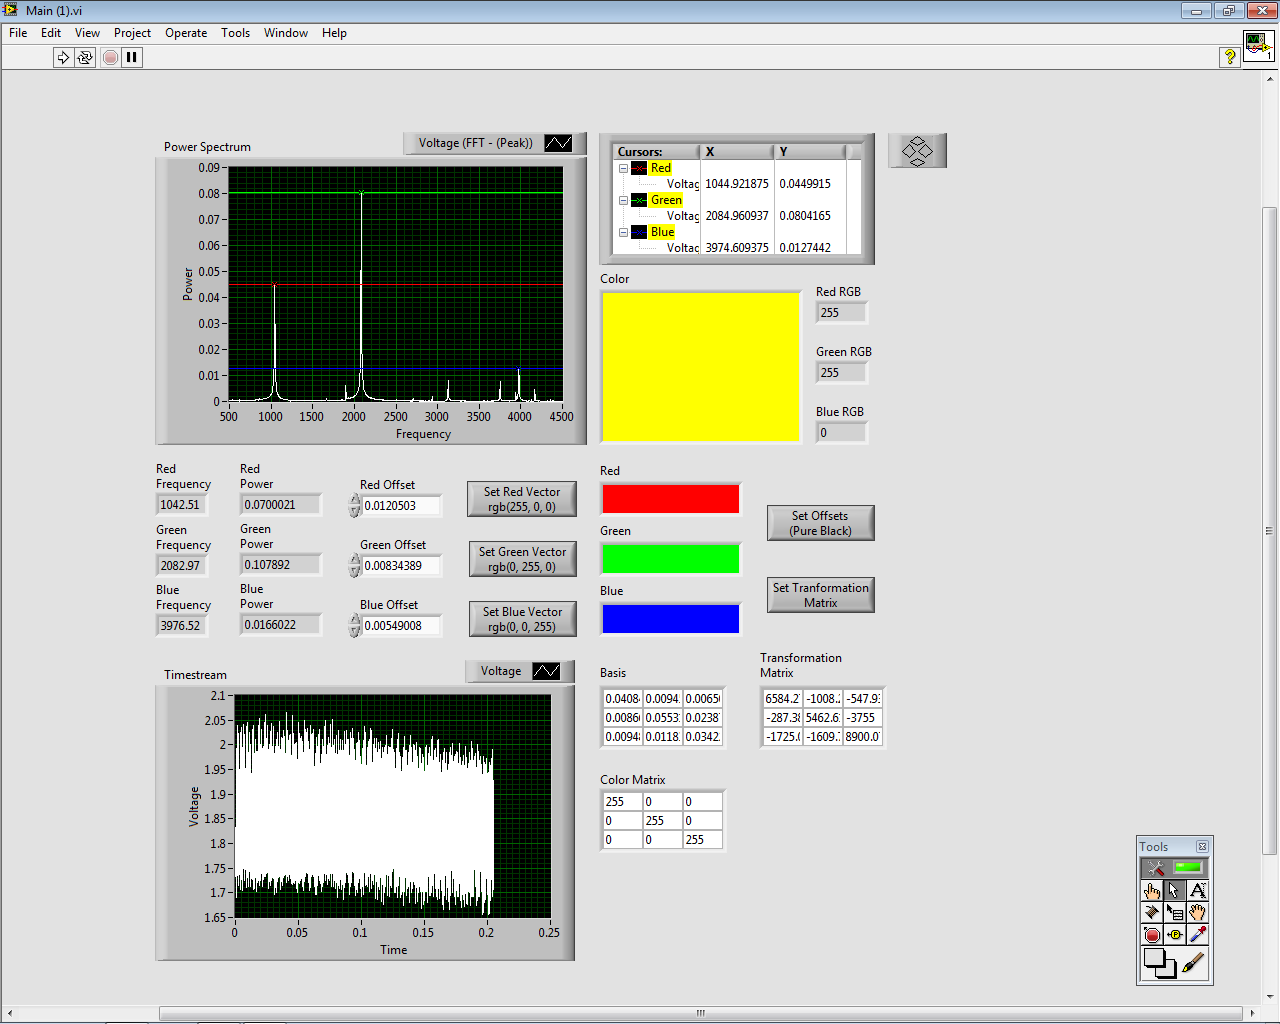
\includegraphics[scale=.4]{front_panel_yellow.png}
\caption{The time stream graph is the raw data as we read in the analog voltages into Labview. the Power spectrum graph displays the RGB signals with very little noise. Finally the basis matrix, color matrix and transformation matrix are used to calibrate the colors and then measure the color of objects. The set RGB vector buttons used to build the basis matrix and the \textit{set offset }button is used to find and subtract the voltage reading when we shine the LED's onto a black surface. That is when there is little to no reflection.}
\label{front}
\end{figure}


\begin{figure}[H]
\centering
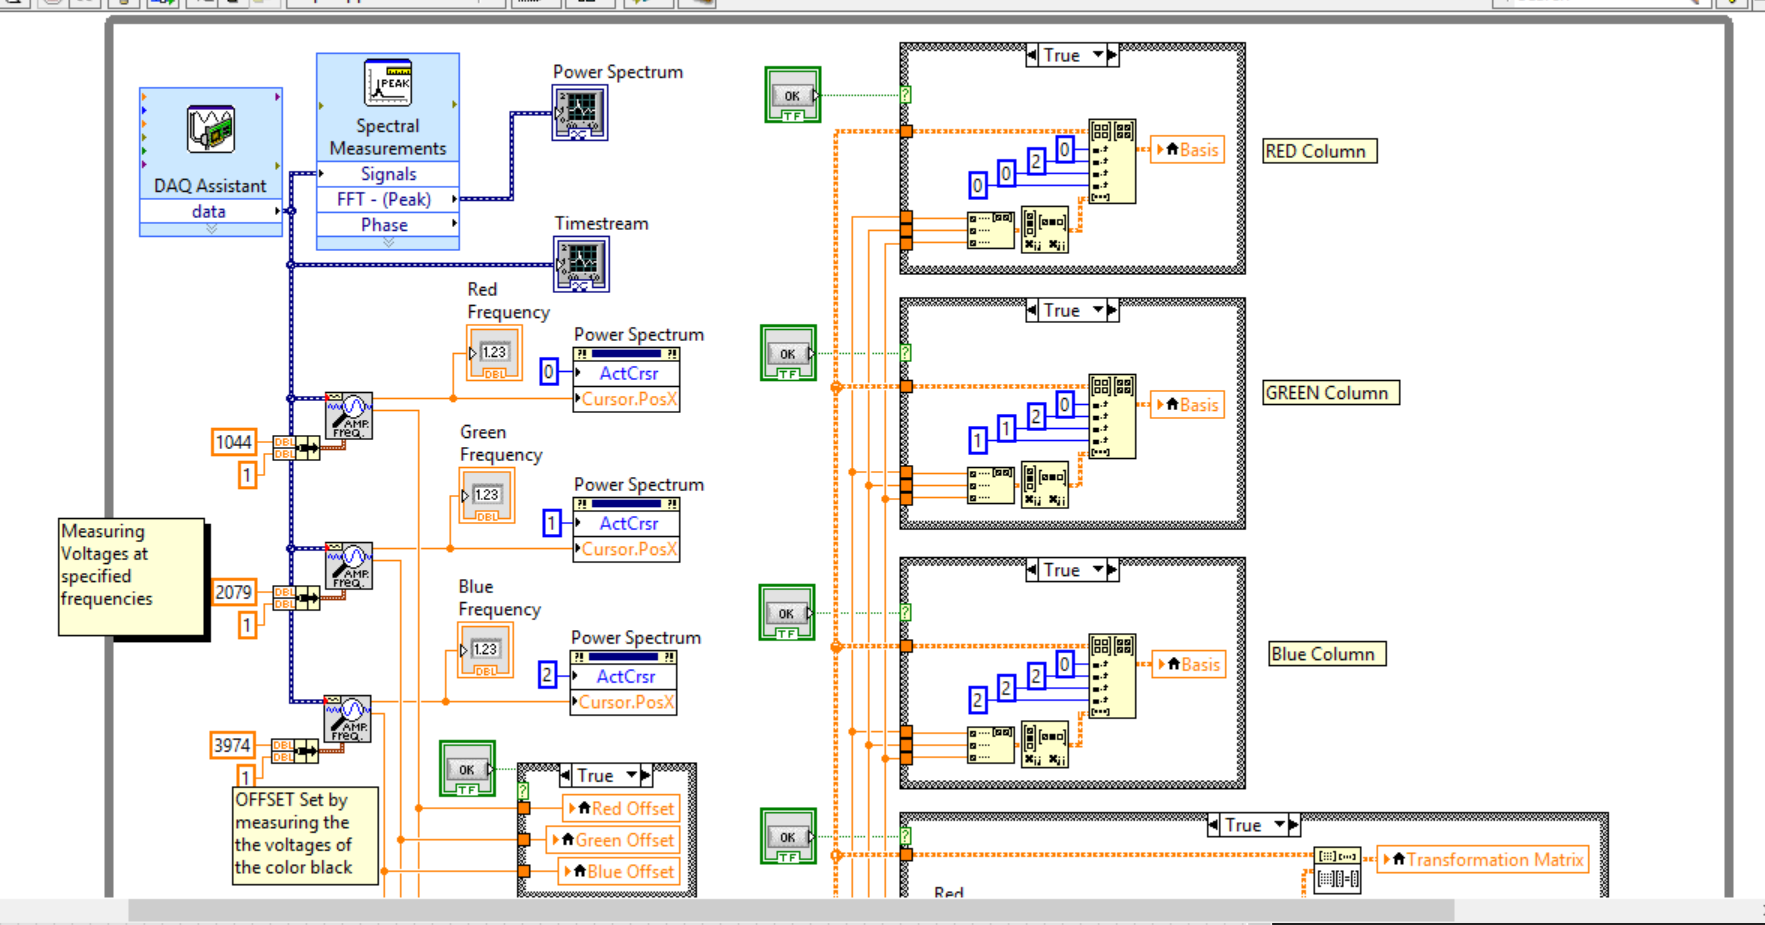
\includegraphics[scale=.4]{backpanel1.png}
\caption{This is an image of our backpanel. The left side of the panel displays the functions we used to read in our data and preform the FFT. It also shows the function used to measure the amplitude voltages at the specified frequencies. The right side of the panel is the function used to build our Basis matrix for the RGB LED's. The Basis matrix is used to find the transformation matrix that will take us from voltage into the color space. The center of the panel also has three constants that are titled Red, green and blue offsets. The offset refers to the voltages measured when we shine the LED's onto a pure black object. this is also used as part of the calibration process.}
\label{backpanel1}
\end{figure}




By knowing the frequency of the red, green and blue LED's, we could extract the voltages at those specific frequencies. we used a built in function called single tone information to read out voltages at those specific frequencies. we then displayed that information in the front panel and also passed on that information into an build matrix function. the build matrix function builds the columns of a 3X3 matrix. each columns belongs to a specific color RGB and each elements is used to build the basis matrix. The first figure of our program is shown in figure \ref*{backpanel1}

After building the basis matrix we then built the standard color space matrix by specifying the vector values which correspond to Red, Green and Blue. 

\begin{figure} [H]
\centering
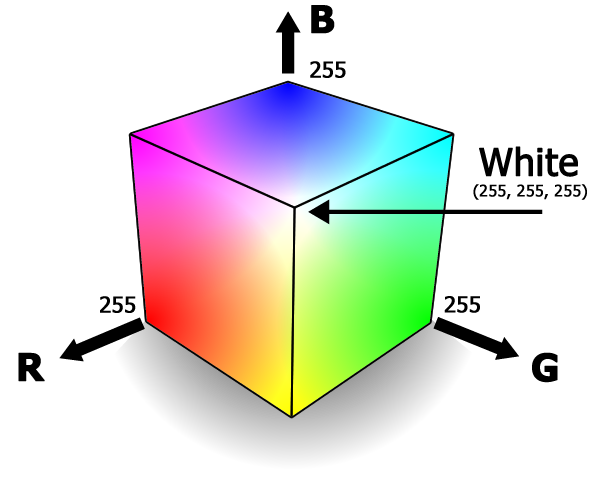
\includegraphics[scale=.2]{color_cube.png}
\caption{Color vector space. The color in the cube are represented with a vector. For example black is (0,0,0) ,red would be (255,0,0), green would be (0,255,0) etc. The range [0,255] are the standard values used to represent colors in the digital world.}
\label{color_cube}
\end{figure}



Finally by using a the basis matrix and the color space matrix we were able to use a function called solve linear equation to find the transformation matrix which will map voltages to color. That is:

\begin{equation}\label{transformation}
A_{volt}X = Y_{RGB}\indent\indent \Rightarrow\indent\indent X = A_{volt}^{-1}Y_{RGB}
\end{equation}


where $Y_{RGB}$ is the color space matrix, $
\left[ {\begin{array}{*{10}c}
   255 & 0  & 0 \\
   0 & 255  & 0 \\
   0 & 0  & 255 \\

 \end{array} } \right]$, and $A_{volt}$ is the basis matrix which is built by measuring the voltage amplitude when we shine the color sensor at a pure Red, Green and blue surfaces. Finally, $X = T(volt)$ the transformation matrix. Note that in the basis matrix we also correct for the initial offset by measuring the amplitudes for RGB when we shine the color sensor at a pure black surface and subtracting out those values from any further measurement. As an example, we printed out a paper which contained a number of colors including the pure red, green and blue. we then shined the color sensor in red, for example, and pressed the  set red vector in the front panel of our program. this sets the first column of the basis matrix. we then do the same for Green and Blue. finally we pressed the set Transformation button, which solve Equation \ref*{transformation}, and complete the calibration process, that is $T(volts) = X $. An example of a basis matrix would be the basis matrix given in figure \ref*{front} which is the matrix given below.

 \begin{equation}
 A_{volt} = 
\left[ {\begin{array}{*{10}c}
   0.0408 & .0094 & 0.0065 \\
   0.0086 & 0.0553  & 0.0238 \\
   0.0094 & 0.0118 & 0.0342 \\

 \end{array} } \right]
 \end{equation}

Finding the transformation matrix is probably the most important portion of the experiment; therefore, we spent a considerable amount of time getting rid of noise and making sure that the signals belonging to RGB had similar and clearly defined amplitudes.

After we found the transformation matrix we added function to our labview program that allowed us to build a vector. The build matrix function in the lower part of our code creates a Row of RGB voltage values. Since we want to create a vector we had to transpose the row. Finally, by multiplying the the measured vector and Transformation matrix matrix we obtain a vector which corresponds to a vector in color space. We then pass on this information into an RGB to color function, which takes in values from 0-255 and converts them in to a color. A detailed image of the second portion of our block diagram is given in figure \ref*{backpanel2}

 	
\begin{figure}[H]
\centering
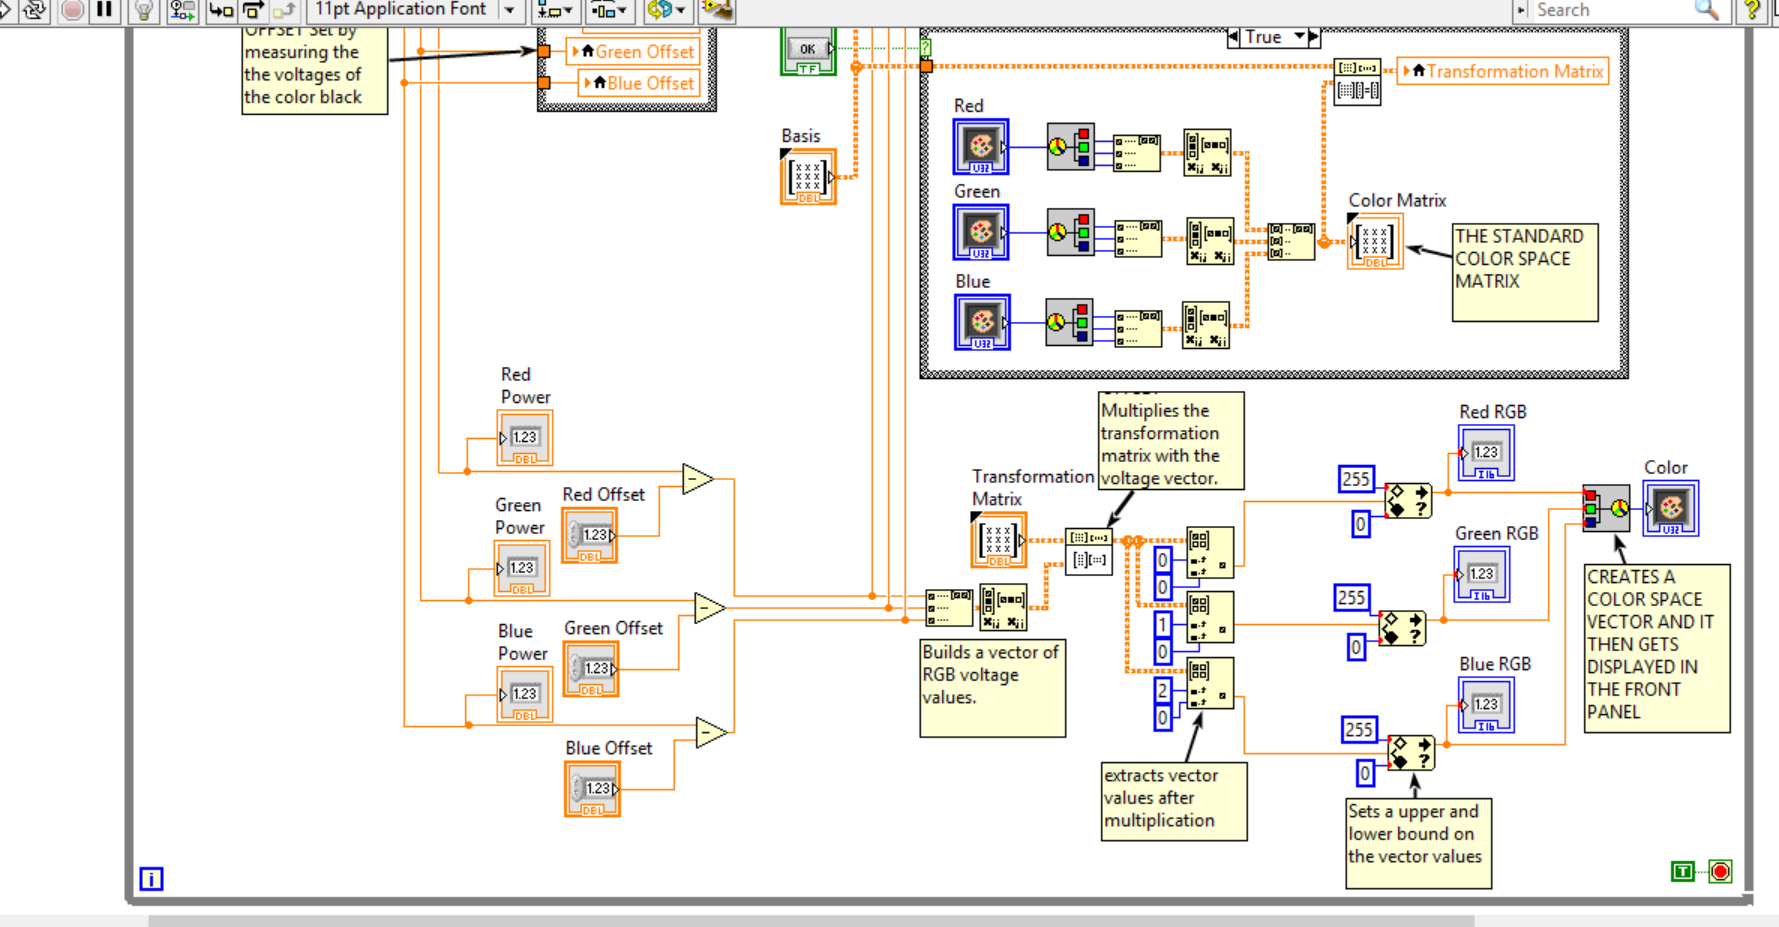
\includegraphics[scale=.4]{backpanel2.png}
\caption{}
\label{backpanel2}
\end{figure}

\section*{RESULTS}

Our color sensor worked better than expected. The dark colors were simple to map to color space, however, the brighter colors required us to make small adjustments to calibration process. As stated earlier we had to reduce noise and amplify the signal. We also had to use high intensity LED's because the low intensities LED's did not calibrate the data properly. We believe this is because the low intensity LED's were not pure in color and although the high intensity LED's weren't either they were closer to the pure colors. Also, the low LED's were not bright enough therefore we could not clearly distinguish signal from noise. After changing to the high intensity LED's were were able to properly map voltages to color. Figure \ref*{testing_sensor} demonstrates how well our color sensor worked.

\begin{figure}[H]
\centering
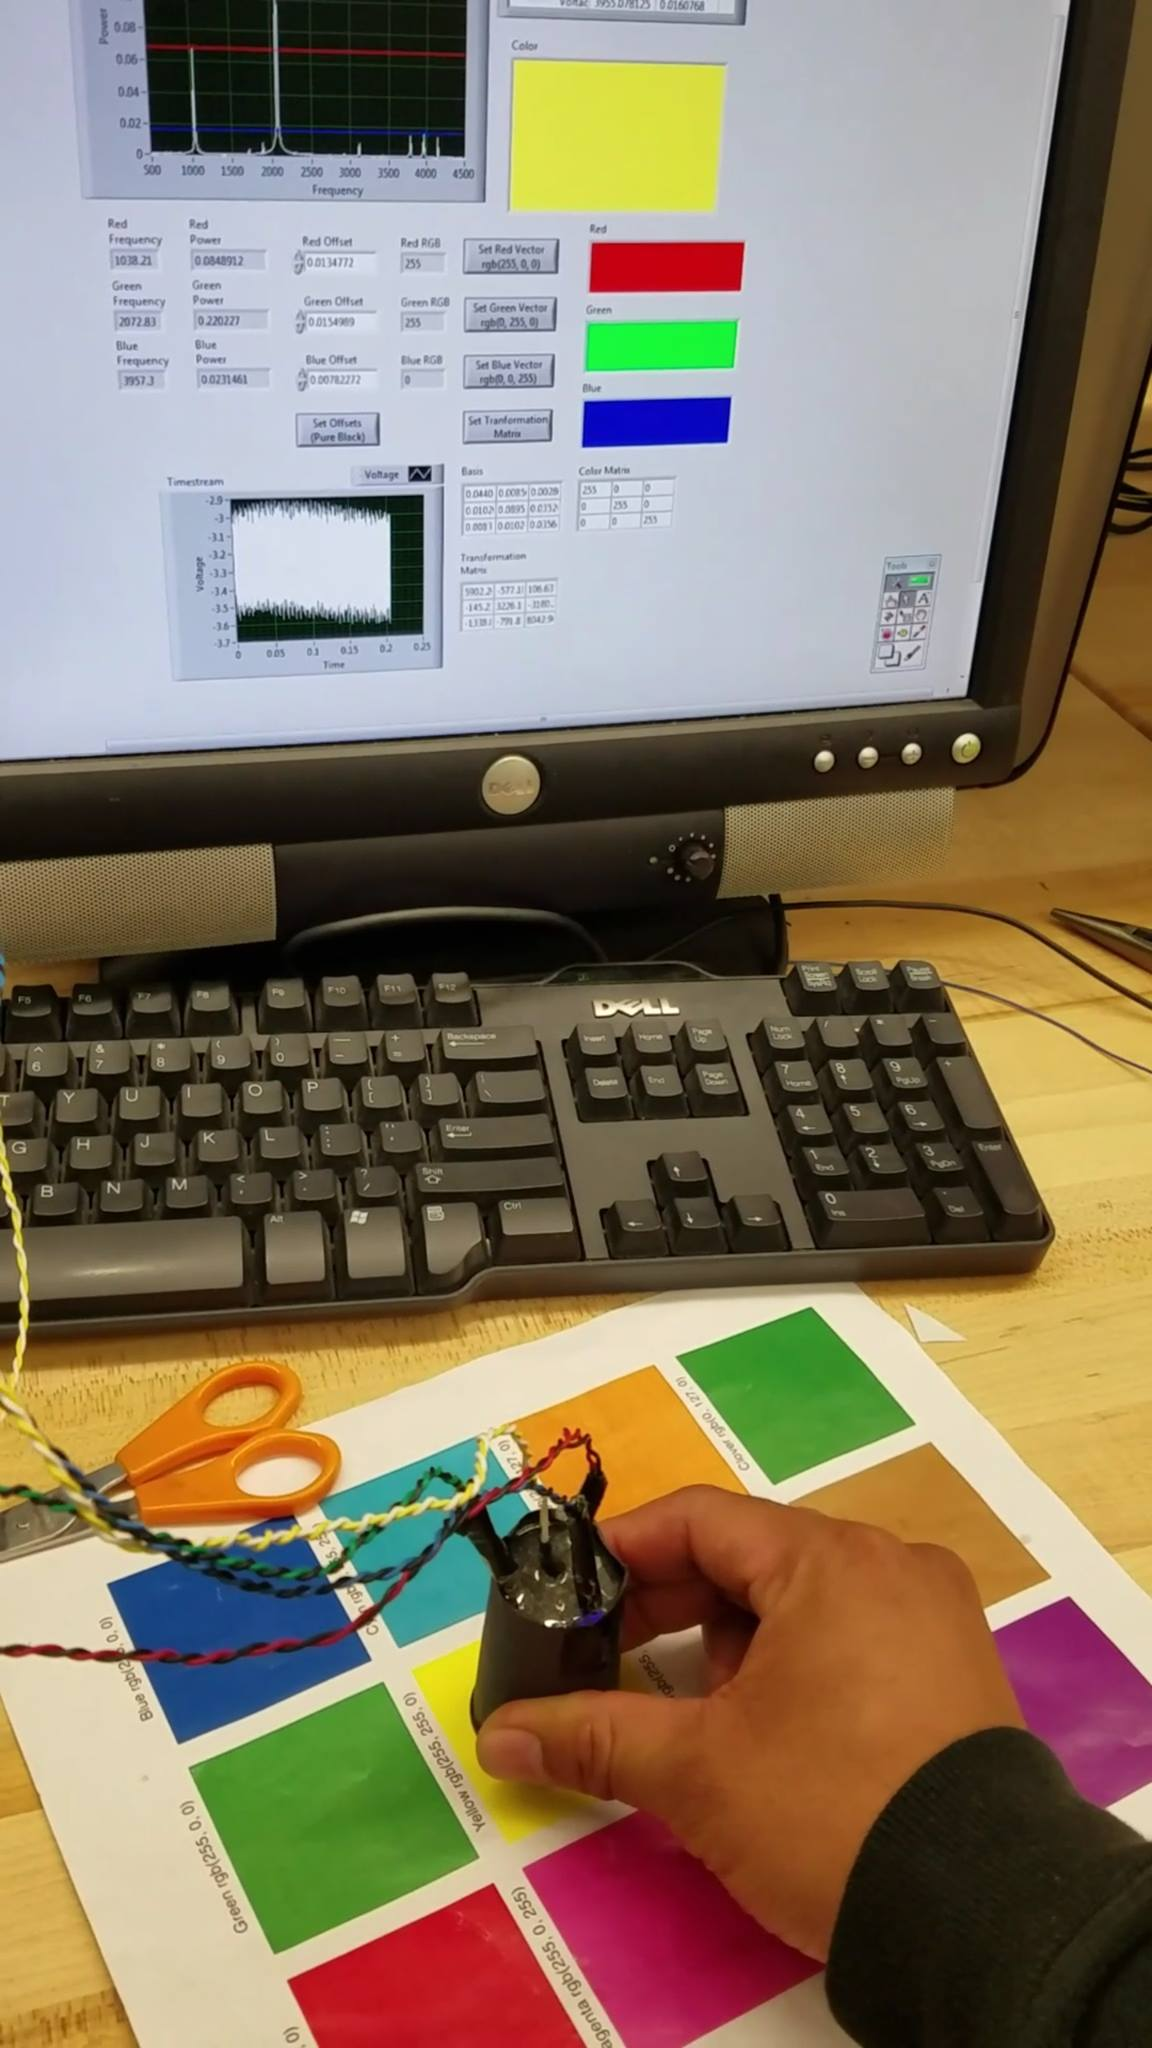
\includegraphics[scale=.2]{testing_sensor.png}
\caption{This figure gives a sample on how our color sensor works. In order to see a video of the color sensor in action copy and paste this link to your internet browser : \url{ https://youtu.be/gj64oGoD7Dk} }
\label{testing_sensor}
\end{figure}



\section*{Conclusion}

In our experiment we set out to understand how spectroscopy works. we did so by building a circuit using a photodiode and three RGB LED's. The photodiode converted light intensity into current. we then used an opamp to convert the current into voltage. The voltage was useful because the DAQ from the lab can read voltages into Labview. our software built a basis matrix which we then used to find the transformation matrix. This allowed us to map voltages into the color space. The issues we ran into when building the hardware and software of our experiment was reducing noise and amplifying the signal. By preforming the necessary calibration we were able to improve our color sensor. Finally, we saw that a proper calibration required us to purchase high intensity LED's. Our results showed that we could map voltages to color in real time. Our color sensor worked so well that our instrument could distinguish colors of different surfaces regardless of how opaque the surface was.




\end{document}